% Capítulo 6 (Resultados) — Slide 3 — Distribuição das séries no plano ADI x CV2 (figura isolada)
\begin{frame}{Distribuição das séries no plano ADI $\times$ CV$^2$}
  \centering
  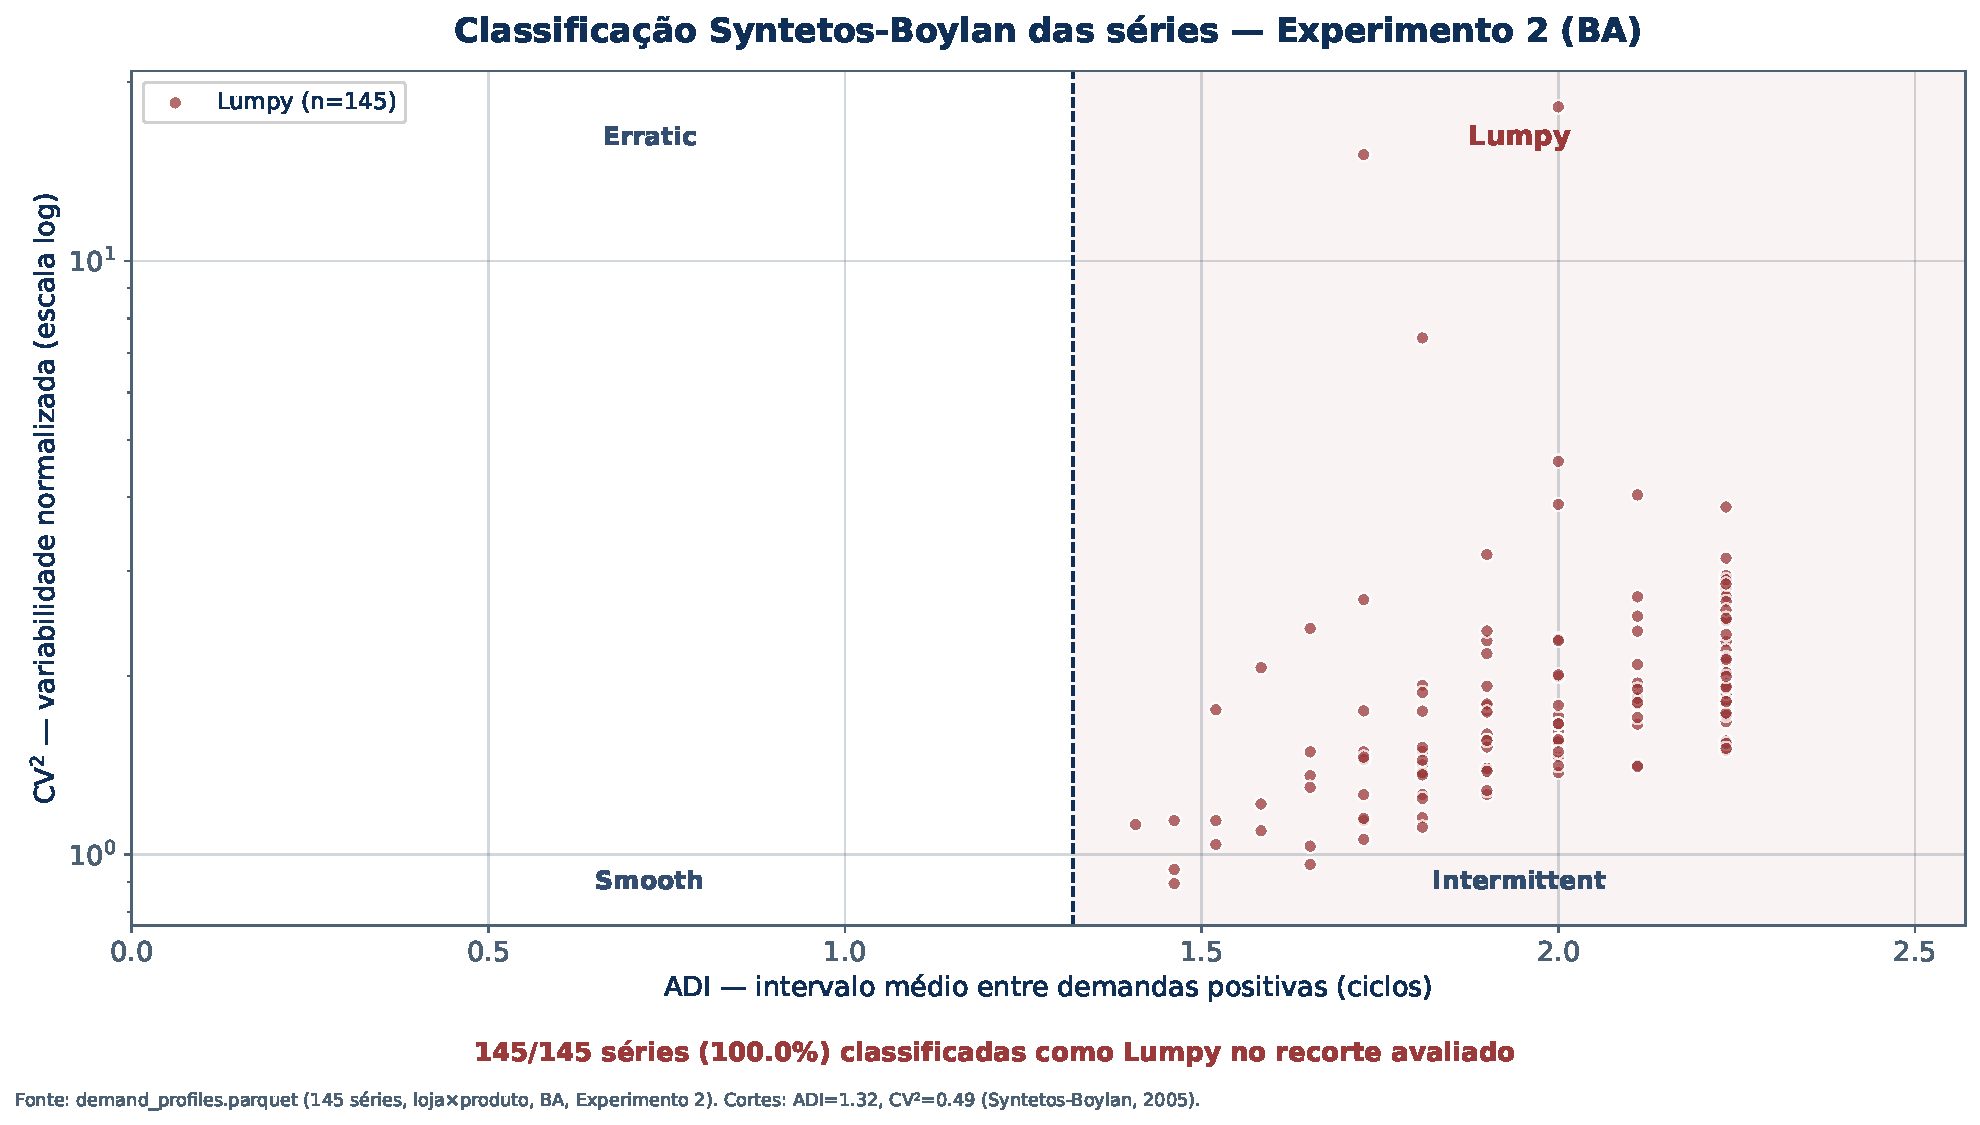
\includegraphics[width=0.86\linewidth,height=7.0cm,keepaspectratio]{figures/syntetos_boylan_scatter.pdf}
  \note{
    Cada ponto é uma série loja-produto, posicionada pelo seu ADI (intervalo
    médio entre demandas positivas) e CV$^2$ (variabilidade normalizada). As
    linhas de corte (ADI=1,32; CV$^2$=0,49) definem os quatro quadrantes da
    taxonomia de Syntetos-Boylan. Neste recorte, as 145 séries avaliadas no
    Experimento 2 foram classificadas no quadrante Lumpy -- o mais desafiador
    para reposição, com longos períodos sem venda intercalados por picos
    irregulares. A predominância de séries Lumpy no recorte avaliado
    justifica o foco em um regime desafiador para reposição: é exatamente
    onde políticas simples têm mais dificuldade e onde a seleção contextual
    de políticas tem mais potencial de fazer diferença.
  }
\end{frame}
